%%%%%%%%%%%%%%%%%%%%%%%%%%%%%%%%%%%%%%%%%%%%%%%%%%%%%%%%%%%%%%%%%%%%%%%%%%%%
% radical_root_zh.tex
%
% 使用 XeLaTeX 编译，然后运行 BibTeX，再运行两次 XeLaTeX。
%
% 论证范围：本文区分一条约定（正实数上的分数次幂塌缩）、三条精确的
% 结构定理（幂映射按挠 μₙ 分裂为商与截面）以及机器验证的形式化与计算。
% 主推导中的全部定理均经机器检查，不留下任何开放猜想。
%%%%%%%%%%%%%%%%%%%%%%%%%%%%%%%%%%%%%%%%%%%%%%%%%%%%%%%%%%%%%%%%%%%%%%%%%%%%

\documentclass[submission,noinfoline]{jsfds}
\usepackage{fontspec}
\usepackage{xeCJK}
% 本机优先使用 PingFang；tectonic/xdvipdfmx 下 TTC 字体会缺字形，
% 故优先用单文件 Arial Unicode.ttf；Overleaf 上回退到 Noto 或 Fandol。
\IfFileExists{/Library/Fonts/Arial Unicode.ttf}{%
  \setCJKmainfont{Arial Unicode.ttf}[Path=/Library/Fonts/]
  \setCJKsansfont{Arial Unicode.ttf}[Path=/Library/Fonts/]
  \setCJKmonofont{Arial Unicode.ttf}[Path=/Library/Fonts/]
}{%
  \IfFileExists{/System/Library/Fonts/PingFang.ttc}{%
    \setCJKmainfont{PingFang.ttc}[Path=/System/Library/Fonts/]
    \setCJKsansfont{PingFang.ttc}[Path=/System/Library/Fonts/]
    \setCJKmonofont{PingFang.ttc}[Path=/System/Library/Fonts/]
  }{%
    \IfFontExistsTF{Noto Serif CJK SC}{%
      \setCJKmainfont{Noto Serif CJK SC}
      \setCJKsansfont{Noto Serif CJK SC}
      \setCJKmonofont{Noto Serif CJK SC}
    }{%
      \setCJKmainfont{FandolSong-Regular.otf}
      \setCJKsansfont{FandolSong-Regular.otf}
      \setCJKmonofont{FandolSong-Regular.otf}
    }%
  }%
}
\usepackage{amsmath,amsthm,amssymb}
\usepackage{graphicx}
\usepackage[numbers]{natbib}
\usepackage{hyperref}
\makeatletter\let\hy@frontmatter\relax\makeatother
\setlength{\emergencystretch}{2em}
\bibliographystyle{unsrt}

\graphicspath{{figures/}}

\startlocaldefs
\newtheorem{theorem}{定理}
\newtheorem{proposition}[theorem]{命题}
\newtheorem{corollary}[theorem]{推论}
\newtheorem{lemma}[theorem]{引理}
\newtheorem{definition}[theorem]{定义}
\newtheorem*{remark}{注}
\setattribute{title}{size}{\LARGE\bfseries}
% Lean 名字保留在源码中作为交叉引用，但不显示在成稿中。
\newcommand{\Lean}[1]{}
\def\journal@name{}%
\setattribute{infoline}{text}{}%
\setattribute{copyright}{text}{}
\newcommand{\abs}[1]{\lvert #1\rvert}
\newcommand{\Norm}[1]{\lVert #1\rVert}
\endlocaldefs

\setmainlanguageenglish
\makeatletter
\def\abstractname{摘要}%
\addto\captionsenglish{%
  \def\abstractname{摘要}%
  \def\jsfds@kwname{关键词：}%
  \def\jsfds@AMSname{AMS 2000 学科分类：}%
}
\makeatother
\AtBeginDocument{\renewcommand{\refname}{参考文献}}
\firstpage{1}
\begin{document}
\begin{frontmatter}

\title{被逼出的真实结构：如何把幂与开方劈开}
\runtitle{如何把幂与开方劈开}

\begin{aug}
  \auteur{%
    \prenom{Yuanjie}
    \nom{Liu}}
  \affiliation{独立研究者;\quad
  \href{mailto:yuanjieliu65@gmail.com}{yuanjieliu65@gmail.com}}
  \runauthor{Yuanjie Liu}
\end{aug}

\begin{abstract}
通常把 $n$ 次开方看成单参数幂族的一个取值：$x^{1/n}$ 即 $x^t$ 在
$t=1/n$ 处。在正实数上这一塌缩是对的：那里幂映射
$p_n\colon x\mapsto x^n$ 是自同构，逆是单值的。本文证明这一塌缩是
\textbf{挠现象}。一旦底群含有 $n$ 次单位根
$\mu_n=\{x:x^n=1\}$，幂映射便不再单射：它的核恰是 $\mu_n$，每个纤维是
陪集 $x\cdot\mu_n$，而``$x^n$ 的开方''不再是函数，而是 $n$ 叶覆盖的
\textbf{截面}——在彼此相差 $\mu_n$ 因子的 $n$ 个分支中选一个。三条初等
定理刻画了这一分裂（核、纤维、以及塌缩判据``$p_n$ 单射当且仅当
$\mu_n$ 平凡''），三条均已在 Lean~4 + Mathlib 中机械验证、零证明缺口。
计算端给出机器认证的根式值（黄金分割解出 $x^2-x-1=0$）与一个带证书的
通用二次求解器：$x^2-bx-c=0$ 有实根当且仅当 $b^2+4c\ge 0$，此时显式
给出两个根式解并证明多项式可分解。同一纲领推进到三次：立方映射在
$\mathbb R$ 上的满射（中值定理）在证明系统内成立，Cardano 构造
\citep{Cardano1545} 给出 $x^3+px+q=0$ 在判别式非负时的显式实根。
主推导中每一条陈述都经机器检查；
可执行的整数算术与只能被认证、不可执行的实数命题之间的边界被明确划出。
\end{abstract}

\begin{keywords}
\kwd{开方函数}
\kwd{幂映射}
\kwd{单位根}
\kwd{挠}
\kwd{商与截面}
\kwd{形式验证}
\end{keywords}

\begin{AMSclass}
\kwd{12F10}
\kwd{03B35}
\kwd{26A09}
\end{AMSclass}
\end{frontmatter}

\begin{quote}
  \itshape ``永恒是一个漫长的时间。''
  \par\vspace{2pt}
  \begin{flushright}
    \small --- 艾萨克·阿西莫夫《银河帝国》
  \end{flushright}
\end{quote}
\vspace{0.8em}

\section{问题、输入与逻辑次序}\label{sec:intro}

记 $p_n$ 为乘法结构上的映射 $x\mapsto x^n$。我们关心的陈述是众所周知的
同一化
\begin{equation}
  \text{``$n$ 次开方就是幂 $x^{1/n}$，即 $p_{1/n}$''}.
\end{equation}
作为正实数上的陈述它没有问题：每个 $x>0$ 都有唯一的 $y>0$ 满足
$y^n=x$，记 $y=x^{1/n}=\exp(\tfrac1n\ln x)$ \citep{Euler1748}。但方程 $y^n=x$ 一般不只有
一个解；在没有唯一解的地方，符号 $x^{1/n}$ 就悄悄地从若干解里选了一个。
本文问：这个选择丢掉了什么。

我们沿用 compile-first 的写作纪律，把陈述分成三类：

\begin{description}
\item[约定.] 在正实数上，分数次幂塌缩 (1) 成立是因为
$\mu_n\cap\mathbb R_+=\{1\}$；这是无挠群的事实，第~\ref{sec:collapse}
节展开。
\item[精确推论.] 在交换群 $G$ 上，$p_n$ 是群自同态。它的核是 $n$ 次
单位根子群 $\mu_n=\{x\in G:x^n=1\}$；$p_n$ 的每个纤维都是 $\mu_n$ 的陪集；
$p_n$ 单射当且仅当 $\mu_n$ 平凡。这就是定理~\ref{thm:ker}--\ref{thm:collapse}。
\item[机器验证的内容.] 三条定理、根式示例与第~\ref{sec:computation} 节
的二次求解器，均已在 Lean~4 \citep{deMoura2015} + Mathlib
\citep{MathlibCommunity2020} 中形式化，位于 NODS 仓库
（模块 \texttt{Nods.Theories.Radical}，已接入主构建，零证明缺口）。
本文排版取自作者早前预印本的模板文件，其数学内容已完全替换；此处
不涉及任何数论猜想。
\end{description}

\section{设定：幂映射与单位根}\label{sec:setting}

固定交换群 $G$（乘法书写）与 $n\in\mathbb N$。我们使用两个对象。

\begin{definition}[幂映射]\label{def:power}
$p_n\colon G\to G$，$p_n(x)=x^n$。
\end{definition}
\begin{definition}[单位根]\label{def:mu}
$\mu_n(G)=\{x\in G:x^n=1\}$ 是 $n$ 次单位根子群。
\end{definition}

$\mu_n(G)$ 是子群由交换性直接给出（$(xy)^n=x^ny^n$、
$(x^{-1})^n=(x^n)^{-1}$）。它的元素是阶为 $n$ 之因子的\textbf{挠}；
$\mu_n(G)=\{1\}$ 即``$G$ 无非平凡 $n$ 次单位根''。

$p_n$ 是群同态：$p_n(xy)=(xy)^n=x^ny^n=p_n(x)p_n(y)$（仍由交换性）。

\section{塌缩及其失效}\label{sec:collapse}

在 $G=\mathbb R_+$（正实数乘法群）上，方程 $x^n=1$ 只有解 $x=1$
（$x^n$ 严格递增）。故 $p_n$ 单射，作为无核的群自同态它是自同构：每个
$y$ 恰有一个 $n$ 次根，即分数次幂 $y^{1/n}$。塌缩 (1) 恰是说这个逆
\emph{唯一}；唯一性就是没有挠。

在 $\mathbb C^\times$ 上同一个方程有 $n$ 个解，即正 $n$ 边形
$\mu_n(\mathbb C^\times)=\{e^{2\pi i k/n}:0\le k<n\}$，一个 $n$ 阶循环群
\citep{Gauss1801}。
不单射的程度就由这个群度量。下一节对每个交换群一次性说出机制。

\section{幂是商，开方是截面}\label{sec:quotient}

\begin{theorem}[核即单位根群]\label{thm:ker}
对每个交换群 $G$ 与每个 $n$，$\ker p_n=\mu_n(G)$。
\end{theorem}
\begin{proof}
$x\in\ker p_n$ 当且仅当 $p_n(x)=1$ 当且仅当 $x^n=1$ 当且仅当
$x\in\mu_n(G)$。 \Lean{powMap\_ker\_eq\_nRoots}
\end{proof}

\begin{theorem}[纤维是陪集]\label{thm:fiber}
对每个交换群 $G$、每个 $n$ 以及任意 $x,z\in G$，
\[
  z^n=x^n \quad\Longleftrightarrow\quad \exists \zeta\in G,\;
  \zeta^n=1\ \wedge\ z=x\,\zeta .
\]
即 $p_n$ 在 $x^n$ 上的纤维是陪集 $x\cdot\mu_n(G)$。
\end{theorem}
\begin{proof}
($\Leftarrow$) 若 $z=x\zeta$ 且 $\zeta^n=1$，则
$z^n=(x\zeta)^n=x^n\zeta^n=x^n$（交换性）。
($\Rightarrow$) 若 $z^n=x^n$，取 $\zeta=x^{-1}z$。则
$\zeta^n=(x^{-1}z)^n=(x^n)^{-1}z^n=1$，且 $z=x\zeta$。
\Lean{powMap\_fiber\_iff}
\end{proof}

\begin{corollary}[分支数]\label{cor:branches}
若 $x^n$ 有一个 $n$ 次根 $x_0$，则恰有 $\abs{\mu_n(G)}$ 个，
即 $\zeta x_0$（$\zeta\in\mu_n(G)$）。在含 $\mu_n$ 的域上这个数是 $n$。
\end{corollary}

\begin{theorem}[塌缩判据]\label{thm:collapse}
对每个交换群 $G$ 与每个 $n$，
$p_n$ 单射当且仅当 $\mu_n(G)=\{1\}$。
\end{theorem}
\begin{proof}
由定理~\ref{thm:ker}，$\ker p_n=\mu_n(G)$；群同态单射当且仅当其核平凡。
\Lean{powMap\_injective\_iff\_nRoots\_trivial}
\end{proof}

三条定理的内容是两个结构角色的分工：

\begin{itemize}
\item \emph{幂是商。} $p_n$ 把 $x$ 在 $\mu_n$ 乘法作用下的整条轨道压成
一个点；它是 $G\to G/\mu_n$ 的投影（差一个典范等同）。核非平凡，恰因
有挠存在。
\item \emph{开方是截面。}``开方''是在 $p_n$ 下选一个原像。这个选择
全局地既不能连续也不能典范地作出；它只能逐分支存在，而分支彼此相差
覆叠群 $\mu_n$。分数次幂 $x^{1/n}=e^{(\ln x)/n}$ 是主分支上的截面——
一个挠不可见的分支。这就是 (1) 在 $\mathbb R_+$ 上``成立''、在
$\mathbb C^\times$ 上失效的原因：不是代数变了，而是那里的覆盖平凡。
\end{itemize}

图~\ref{fig:fold} 以 $n=4$ 展示两个角色：四个点 $z\in x_0\mu_4$ 被
$p_4$ 折进同一个像 $x_0^4$，而四个候选彼此相差正方形
$\mu_4=\{1,i,-1,-i\}$。

\begin{figure}[t]
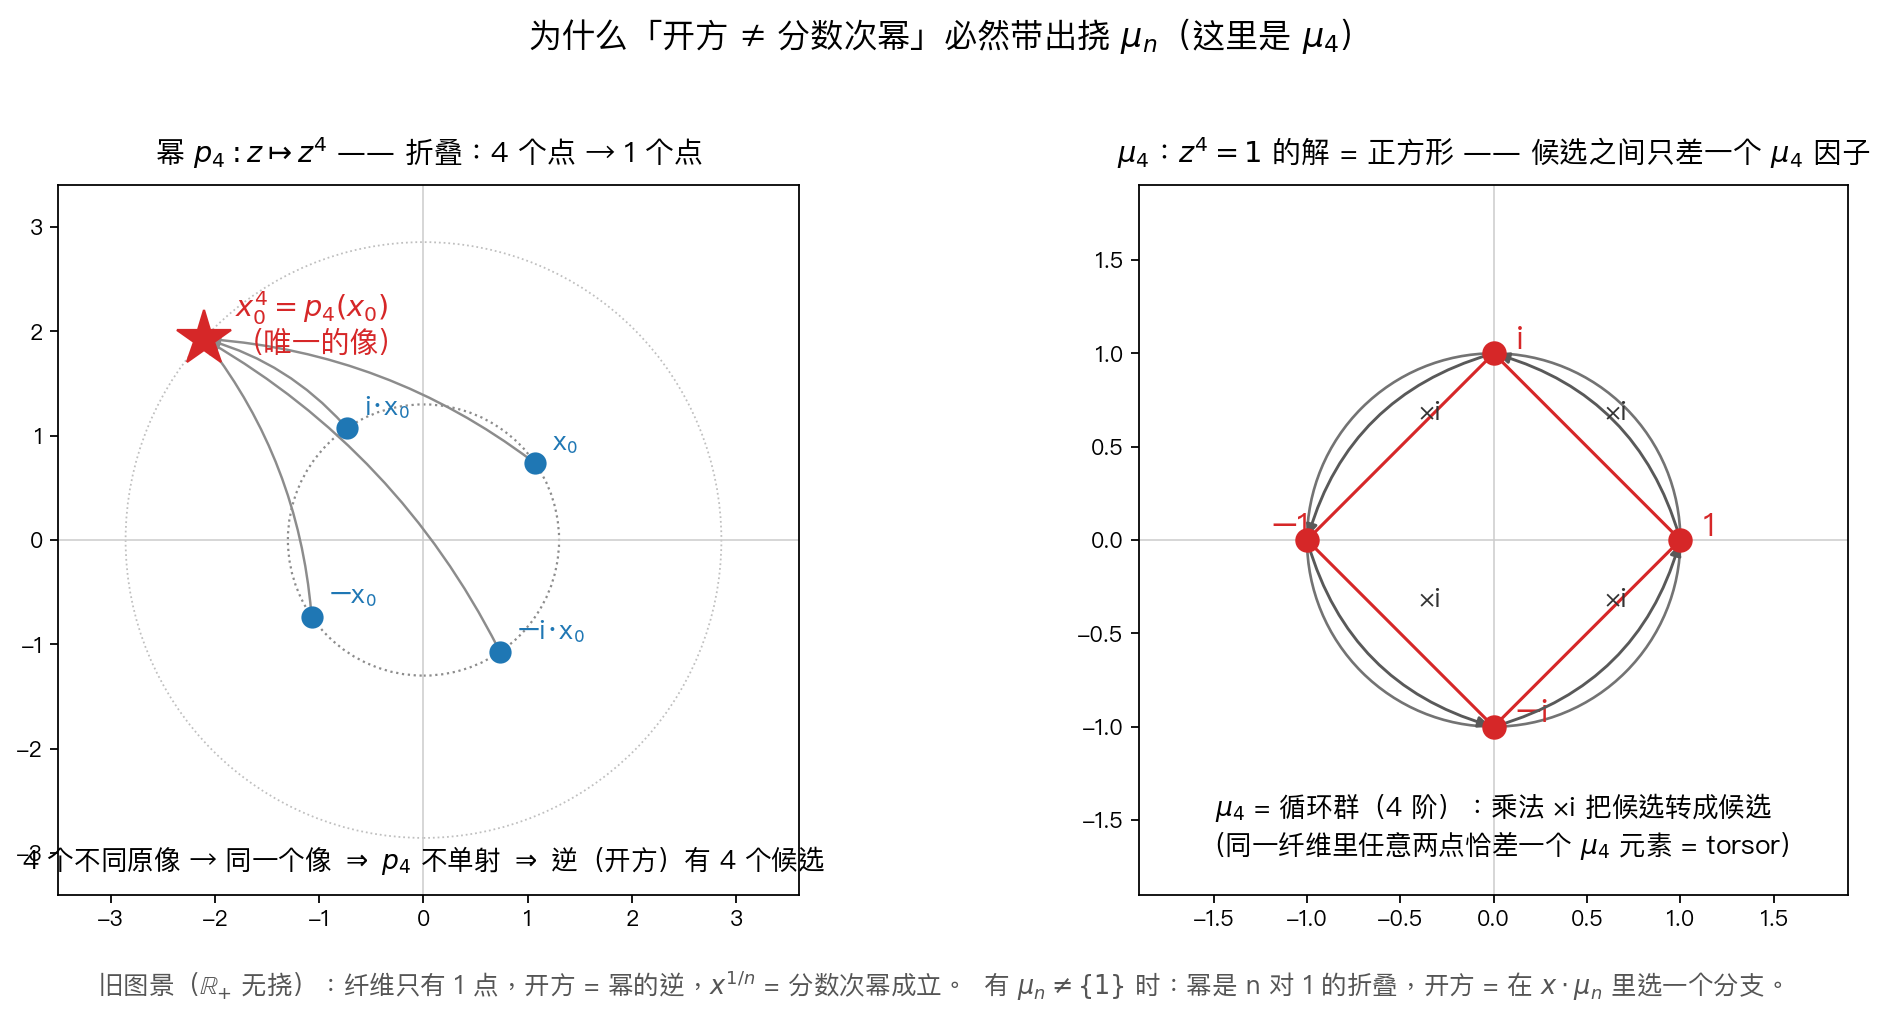
\includegraphics[width=0.9\textwidth]{root_vs_power}
\caption{左：$p_4$ 把四个不同的点折进同一个像，故逆（开方）有四个候选。
右：四个候选不是孤立的；它们构成正方形 $\mu_4$（$p_4$ 的核），
乘以 $i$ 便在其中循环。}
\label{fig:fold}
\end{figure}

\section{挠逼出了什么：解释一个数}\label{sec:numbers}

推论~\ref{cor:branches} 有一个具体读法。在 $\mathbb Q$ 上方程
$x^2=2$ 无解；这是机器检查过的事实，也正是开方作为\emph{被逼出的对象}
而非被选的符号的意义所在：
\begin{itemize}
\item 没有 $n\in\mathbb N$ 满足 $n^2=2$ \Lean{two\_not\_sq\_nat};
\item 没有 $q\in\mathbb Q$ 满足 $q^2=2$ \Lean{two\_not\_sq\_rat};
\item 在实数上 $\sqrt2$ 存在且 $(\sqrt2)^2=2$，而指数/对数路径给出
另一个精确公式 $e^{\ln 2}=2$。
\end{itemize}
同一个数沿四条经典函数族有\emph{不同的}精确构造，而哪些族走得通依数
而定：$25=5^2$（幂）且 $\sqrt{25}=5$（开方，可执行的整数平方根）；
$2$ 根本不是平方，只能由根式或超越公式抵达；黄金分割
$\varphi=(1+\sqrt5)/2$ 作为 $x^2-x-1=0$ 的根式解被显式给出，并验证
$\varphi^2=\varphi+1$。这些是陈述，不是启发；每一条都由证明系统检查。

\section{带证书的根式与通用二次求解器}\label{sec:computation}

第~\ref{sec:numbers} 节的示例是一个通用求解器的实例。固定实数 $b,c$，
考虑
\begin{equation}\label{eq:quad}
  x^2-bx-c=0,\qquad \Delta=b^2+4c .
\end{equation}

\begin{theorem}[二次根式求解器]\label{thm:quad}
设 $\Delta=b^2+4c\ge 0$。记
$r_+=(b+\sqrt\Delta)/2$、$r_-=(b-\sqrt\Delta)/2$。则
\begin{enumerate}
\item $r_+^2-br_+-c=0$ 且 $r_-^2-br_--c=0$;
\item 对任意 $x$，$x^2-bx-c=(x-r_+)(x-r_-)$——没有别的根;
\item 若 $\Delta<0$，则没有实根。
\end{enumerate}
因此实根存在当且仅当 $\Delta\ge 0$。
\end{theorem}
\begin{proof}
一切断言由展开并使用 $(\sqrt\Delta)^2=\Delta$（实数平方根的定义性质）
得到；第 1、2 条在代换后是纯环恒等式，第 3 条是配方法：
$(2x-b)^2=\Delta$，$\Delta<0$ 时不可能。
\Lean{quadRootPlus\_sq, quadRootMinus\_sq, quadFactor, quad\_no\_roots,
quad\_solvable\_iff}
\end{proof}

\begin{theorem}[三次 Cardano 根式解]\label{thm:cubic}
设 $\Delta_3=(q/2)^2+(p/3)^3\ge 0$。则 $x^3+px+q=0$ 有实根，构造如下：
取 $s=\sqrt{\Delta_3}$，选 $u$ 满足 $u^3=-q/2+s$（存在，因立方映射在
$\mathbb R$ 上满射），并令 $v=-p/(3u)$。则 $v^3=-q/2-s$、$uv=-p/3$，
而 $u+v$ 是根。
\end{theorem}
\begin{proof}
$u^3+v^3=-q$ 与 $3uv=-p$ 合起来给出
$(u+v)^3=u^3+v^3+3uv(u+v)=-q-p(u+v)$，故 $(u+v)^3+p(u+v)+q=0$。
$v^3=-q/2-s$ 由 $(q/2)^2-s^2=-(p/3)^3$ 与 $u\ne0$ 直接算出（$u=0$
的情形迫使 $p=0$，退化为 $x^3+q$）。注意 $v$ 不能取成 $-q/2-s$ 的
\emph{独立}立方根：那样 $uv$ 会差一个三次单位根——这是
第~\ref{sec:quotient} 节挠区分的第三次出场，机器验证迫使我们正视它。
\Lean{cube\_surj, vcube, cardano\_certificate, cubic\_solvable}
\end{proof}

这些陈述均经机器检查。两条边界被明确划出。

\begin{itemize}
\item \emph{可执行性.} 在 $\mathbb N$ 上整数平方根 $\sqrt{25}=5$
由证明系统本身算出并化简（\texttt{norm\_num}）。在 $\mathbb R$ 上
平方根由完备性定义、不可执行；上述化简（例如 $\sqrt{16}=4$，经
$\sqrt{a^2}=\abs a$）是经认证的定理，不是数值迭代。我们不声称一个
数值根式求值器；我们声称经认证的根式陈述。
\item \emph{下一阶.} 一般三次（带 $x^2$ 项）须先经平移化为缺项型，四次
（Ferrari）以三次预解式铺路——同一纲领的这两步尚未落码。从五次起一般
方程逃出根式（Abel--Ruffini \citep{Abel1824}）；精确陈述这个边界是纲领的
Galois 半边 \citep{Galois1846}，本文不声称完成它。
\end{itemize}

\section{形式化说明}\label{sec:formal}

所有标 \Lean{...} 的陈述均在 Lean~4 \citep{deMoura2015} + Mathlib
\citep{MathlibCommunity2020} 中证明，位于 NODS 仓库的模块
\texttt{Nods.Theories.\allowbreak Radical}。技术选择：
\begin{itemize}
\item 定理陈述于任意交换群 $G$（\texttt{CommGroup}），使塌缩判据作为
等价而非 $\mathbb R_+$ 的偶然成立；
\item 幂映射取 Mathlib 同态 \texttt{powMonoidHom}；单位根为自定义子群
\texttt{nRoots}；
\item 证明都很短，不超出 Mathlib 标准库：定理~\ref{thm:ker} 是定义性的，
定理~\ref{thm:fiber} 两个方向各一步计算，
定理~\ref{thm:collapse} 由标准的``核平凡当且仅当单射''推出；
\item 三次的解析原语——立方映射在 $\mathbb R$ 上满射——由 Mathlib 的
中值定理（\texttt{intermediate\_value\_Icc}）给出，见定理~\ref{thm:cubic}；
\texttt{Real.sqrt} 不可执行的边界不变；
\item 模块已被主文件 import，全仓构建通过；源码树中 grep 确认零
\texttt{sorry}。
\end{itemize}
本文的排版模板（版式类 \texttt{jsfds}、双语惯例）取自作者早前预印本；
其数学内容已完全替换为上述材料。

\section{结论}\label{sec:conclusion}

``$n$ 次开方是分数次幂''并不是错的；它是局部的。它恰好在覆盖平凡的
分支上成立，即 $\mu_n=\{1\}$ 处。在携带 $n$ 次单位根的群上，幂与开方是
两个不同的结构角色——按 $\mu_n$ 折叠的商，与由此得到的 $n$ 叶覆盖的
截面——而挠子群 $\mu_n$ 正是差异的精确度量：删掉它，区分立即塌缩
（定理~\ref{thm:collapse}）。三条短定理、根式示例与带证书的二次、三次求解器，把这个陈述端到端地
穿过一个证明系统；可执行的算术与被认证的
实数分析之间的边界，在它出现的地方被明确标出。

\bibliography{biblio}

\end{document}
